%----------------------------------------------------------------------------
\chapter{A Jporta}\label{chapter:jporta}
%----------------------------------------------------------------------------

A Jporta a Budapesti Műszaki és Gazdaságtudományi Egyetem (továbbiakban: BME) Irányítástechnika és Informatika Tanszékén (továbbiakban: IIT) működő, a BME Közigazgatási Informatikai Központ (továbbiakban: BME IK vagy IK) által fejlesztett, oktatást támogató portál, mely a fő funkcióját képző feladatbeadó és -kiértékelő rendszeren kívül az oktatással kapcsolatos adminisztrációs feladatokban (pl. jelenlét vezetése, hallgatók értékelése, üzenetváltás felhasználók között) is segíteni igyekszik felhasználóit.

Ugyan a Jporta fejlesztése csak 2013-ban kezdődött, a tanszéken már 2008 óta használják az eredetileg prototípusnak készült Cporta rendszert, mely minden szempontból a Jporta elődjének tekinthető.

\section{Cporta -- a prototípus}
A Cporta feladatbeadó és gyakorló rendszer a nevéhez illően kifejezetten a C és C++ nyelvek oktatásához lett kifejlesztve.
A portálon a hallgatóknak lehetősége van a kiadott feladatokra C és C++ nyelven íródott programkódok feltöltésére, melyeket a rendszer lefordít, futtat, és teszteléssel értékel.
Lehetőség van emellett fordítást nem igénylő fájlok feltöltésére is (pl. dokumentáció, bemeneti fájlok a teszteléshez).
A Cporta ezen kívül tanulmányi rendszer jellegű funkciókat is megvalósít: kezeli a hallgatók eredményeit és a jelenléti íveket is.
\cite{Ory13}
\begin{figure}
    \centering
    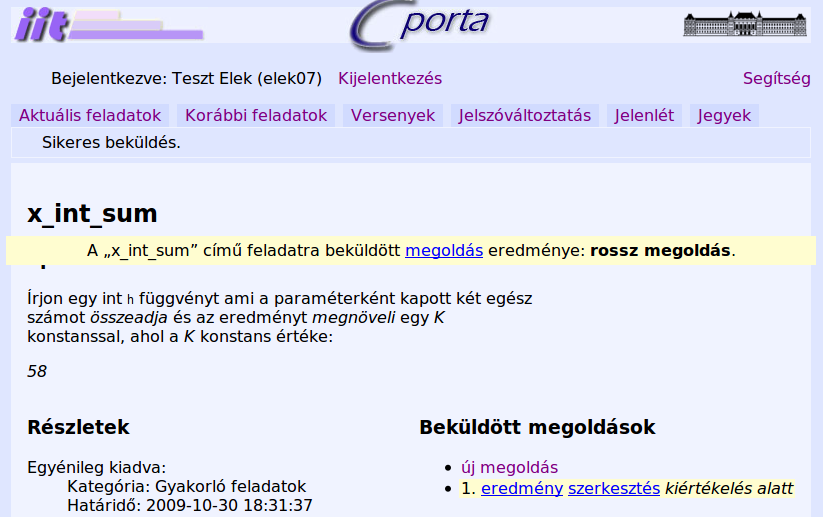
\includegraphics[width=\textwidth]{figures/Cporta}
    \caption{A Cporta felülete}
\end{figure}
Ezeket a funkciókat a Jporta bevezetéséig továbbra is a Cporta látja el \textit{A programozás alapjai 2.} tárgy esetében.

\subsection{A Cporta működése}
A Cportán -- ahogy az oktatásban általában -- a feladatokat az oktatók készíthetik el.
A feladatok több részből állnak:
\begin{itemize}
    \item metaadatok (cím, szerző, fordítási paraméterek, futtatási korlátozások, stb.),
    \item specifikáció (a feladat leírása HTML formában),
    \item oktató által megadott fájlok,
    \item tesztesetek.
\end{itemize}
A feladat specifikációja lehet statikus, vagy a hallgató adatai alapján dinamikusan generált, így lehetőség van hasonló, ám hallgatónként egyedi feladatok készítésére.
Az oktató által megadott fájlok lehetnek nyilvánosak (pl. a használható függvények fejléceit tartalmazó állomány), vagy rejtettek (pl. a teszteléshez használt bemeneti adatfájlok).
A tesztesetek a fordítási lépés eredményeként kapott futtatható állományon hajtódnak végre.
A specifikációhoz hasonlóan kétféle változatuk lehetséges.
Egyszerűbb esetben megadhatunk egy statikus bemenetnél elvárt statikus választ vagy kilépési kódot, amit a teszteset ellenőriz.
Összetettebb esetben megadhatunk két futtatható parancsállományt: az egyik előkészíti a futtatási környezetet és a szabványos bemenetet, a másik ellenőrzik a futás utáni környezetet, kimenetet és kilépési kódot.
\cite{Ory13}

A kiadott feladatokra a hallgatók megoldásokat küldhetnek be, melyeket a rendszer a lehető leghamarabb kiértékel.
A megoldások tartalmazhatnak C és C++ nyelvű forrásállományokat, a tesztelés során elérhető adatállományokat, illetve dokumentációs fájlokat.
A webportálra feltöltött megoldások egy központi ütemezőn keresztül kerülnek a kiértékelést végző végrehajtó gépre.
A kiértékelés végén a végrehajtó gép az eredményeket visszaküldi a webportálra, amely megjeleníti azokat a felhasználóknak. 

A Cporta eredetileg az online, elektronikus feladatkiadás és -beadás oktatásban való használatának vizsgálatára, a koncepció működésének bizonyítására készült.
Ez a prototípus azonban nem hosszútávú használatra lett tervezve, továbbá a használat során felmerülő igényekre válaszként tervezett és beépített kiegészítések a fejlesztésükre szánt idő és erőforrások hiányában -- és ebből következően megfelelő tesztelés és dokumentáció nélkül -- rontották a rendszer stabilitását és karbantarthatóságát.  
A portál üzemeltetését végzők egyöntetű döntése nyomán 2013-ban elindult a Cporta utódjának fejlesztése, eredetileg \textit{swd} néven.

\section{Jporta -- válasz az igényekre}
A Jporta fejlesztésekor az összes Cportával megszerzett tapasztalat a fejlesztők rendelkezésére állt.
A fejlesztéseket 2013-ban Őry Máté kezdte meg szakdolgozata részeként, melyben részletesen elemezte a régi rendszer hiányosságait és az új rendszerrel szemben támasztott követelményeket (lásd \cite{Ory13}).
Munkája részeként ezek alapján megtervezte és elkészítette az új rendszer pilot változatát.  
Ez a változat a feladatkiértékelő funkciónak egy, a Cportáéhoz hasonló, egyszerű változatát valósította meg.
A munka értékelésekor a projekt vezetői arra a döntésre jutottak, hogy a pilot feladatkiértékelő funkciójának felépítése túlságosan merev, néhány használati eset megvalósítására nem, vagy csak nehezen alkalmas. 
Ekkor a portál fejlesztését az IK Cloud csapatának tagjai -- köztük jómagam -- vették át.
Az én feladatom a feladatok leírását és kiadását, és az azokra érkező megoldások beadását és értékelését lehetővé tevő modul továbbfejlesztett modelljének kidolgozása lett, míg a felhasználói felület és az egyéb adminisztrációs funkciók tervezését és implementációját Kálmán Viktor végezte (lásd \cite{Kalman14}).

Az Őry Máté által újratervezett portál sok tekintetben szakított a Cportában felhasznált technológiákkal.
Az új rendszer implementálásához a Python programnyelv 2-es változatát válaszotta, melyet a későbbiekben a 3-as változatra frissítettünk, ezzel biztosítva a szoftver alapját képző komponens tartós támogatottságát. \cite{PEP373} \cite{Kalman14}
A portál második alapja a Django webes keretrendszer\footnote{A dolgozat írásának pillanatában a portál a Django 1.8.9-es verzióját használja.}, mely a webes felület generálásáért és a belső adatmodellen végzett műveletek adatbázisműveletekre fordításáért és végrehajtásáért felel. 
A teljes projekt megannyi más technológiát is felhasznál, amelyek nem kapcsolódnak szorosan ezen dolgozat témájához.
A feladat szempontjából fontos, az implementációban alkalmazott technológiákat a \ref{chapter:exercise}. fejezet külön tárgyalja.

\section{A portál használata}
Ahogy azt az előzőekben láthattuk, a portál sok szolgáltatást nyújt felhasználói számára. 
Ezeket a felhasználókat 4 csoportra oszthatjuk: vendégek (nem azonosított felhasználók), hallgatók, oktatók, illetve az adminisztrátorok.
Mivel a tanszéken sok doktorandusz és demonstrátor is végez oktatási tevékenységet, egy felhasználó szerepelhet bizonyos tárgyaknál oktatóként, míg másoknál hallgatóként.
A portál vendégek számára -- jelenleg -- nem tartalmaz hozzáférhető tartalmat, így a még be nem jelentkezett felhasználókat a belépőoldal fogadja.
A belépőoldalon a felhasználók azonosítására két lehetőség van: eduID (egyetemi \underline{s}ingle \underline{s}ign-\underline{o}n) vagy a hagyományos felhasználónév--jelszó páros (lásd \figref{jporta-login}).
\begin{figure}[h]
    \centering
    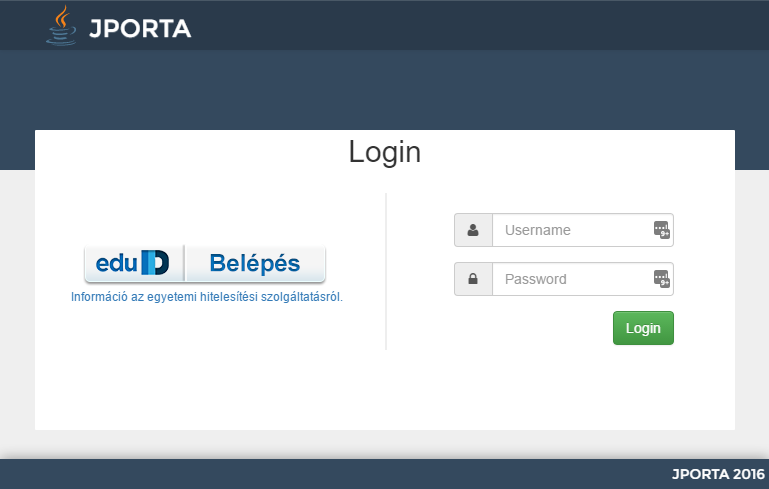
\includegraphics[width=\textwidth]{figures/Jporta-login}
    \caption{A Jporta belépőoldala}
    \label{figure:jporta-login}
\end{figure}
Belépés után a felhasználókat egy kezdőoldal fogadja, melyen a fontosabb információk (pl. aktív és korábbi feladatok, kézi beavatkozást igénylő feladatok) gyűjteménye található.
Már a kezdőoldalon látható (\figref{jporta-home-h}, \figref{jporta-home-o}), hogy a különböző felhasználói szerepek különböző funkciókat tesznek elérhetővé a rendszerben.
Mivel ezek az eltérések egy adott felhasználói szerepkörre (hallgató, oktató, adminisztrátor) jellemzőek, ezért ezeket a nézöpontokat és a hozzájuk kapcsolódó funkciókat az alábbiakban külön részletezem.

\subsection{A portál használata hallgatói szemszögből}
A portálra belépő hallgatókat korábbi és aktuális feladataik listája fogadja (\figref{jporta-home-h}).
Az egyes feladatok mellett található linkekre kattintva eljutnak a feladatok oldalára, ahol megtekinthetik a feladatra beadott előző megoldásaikat, illetve újabb megoldást adhatnak be.
\begin{figure}[h]
    \centering
    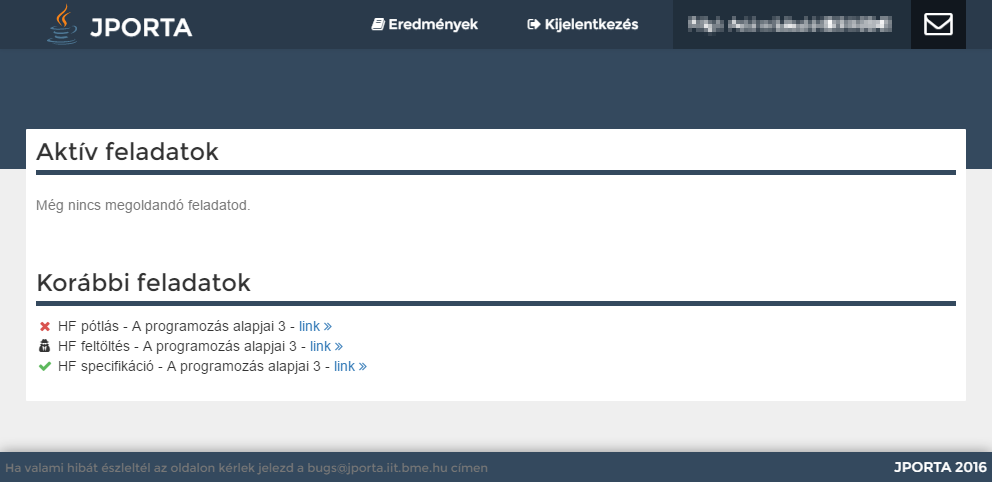
\includegraphics[width=\textwidth]{figures/Jporta-home-h}
    \caption{Jporta kezdőlap (hallgató)}
    \label{figure:jporta-home-h}
\end{figure}

A fejlécben található \textbf{Eredmények} gombra kattintva eljuthatnak egy másik oldalra (\figref{jporta-results}), ahol az értékeléseikről -- a feladatoktól eltérő, pl. zárthelyi dolgozat eredménye -- és a katalógusos órákon való jelenlétükről kapnak információt.
\begin{figure}[h]
    \centering
    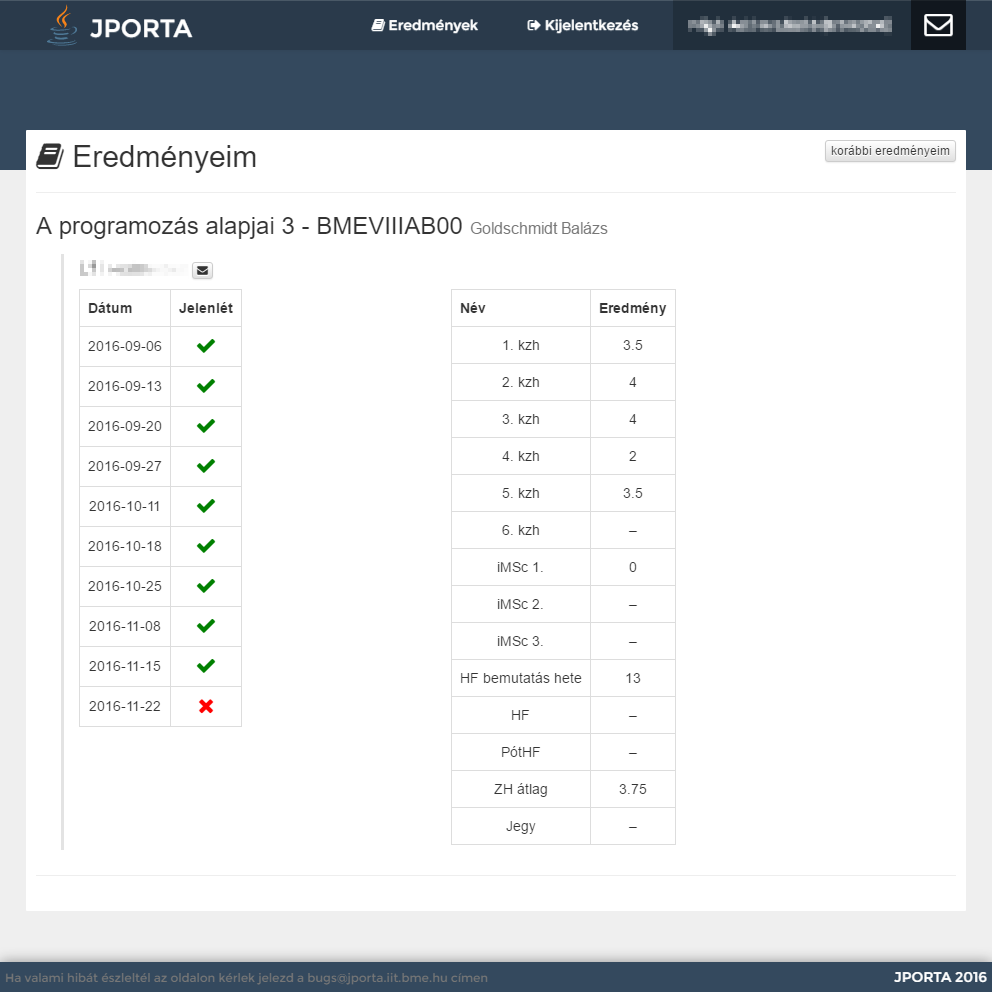
\includegraphics[width=\textwidth]{figures/Jporta-results}
    \caption{Eredményeim oldal}
    \label{figure:jporta-results}
\end{figure}

A portál használata ennyiben lényegében ki is merül a hallgatók számára, eltekintve néhány további közös funkciótól, melyeket a szakasz végén részletezek.

\subsection{A portál használata oktatói szemszögből}
A portálra belépő oktatókat a figyelmüket igénylő beadások listája fogadja, melyeknél oktatói beavatkozás szükséges.
A beadás linkjére kattintva eljutnak annak részletező oldalára, ahol elbírálhatják a megoldás helyességét.
\begin{figure}[h]
    \centering
    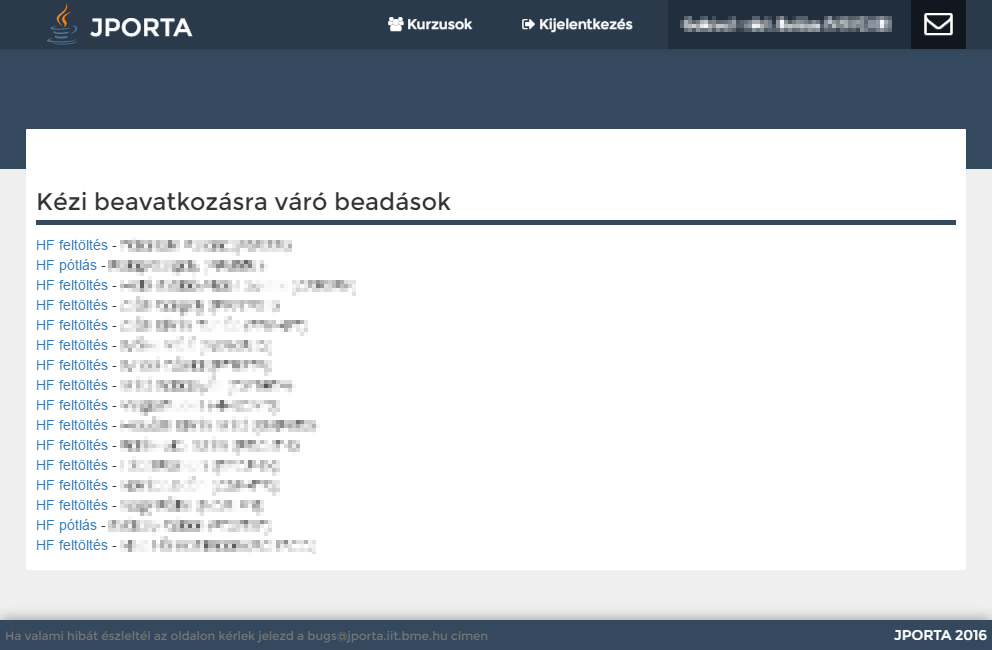
\includegraphics[width=\textwidth]{figures/Jporta-home-o}
    \caption{Jporta kezdőlap (oktató)}
    \label{figure:jporta-home-o}
\end{figure}

A fejlécben található \textbf{Kurzusok} gombra kattintva eljuthatnak az általuk oktatott kurzusokat prezentáló oldalra.
Itt egy konkrét kurzust kiválasztva annak részletező oldalára kerülnek.
Ezen az oldalon különböző füleken megtekinthetőek és módosíthatóak:
\begin{itemize}
    \item a kurzus adminisztrátorai,
    \item a kurzus tagjai (oktatók és hallgatók is),
    \item a kurzusnak kiadott feladatok,
    \item a kurzus eseményei,
    \item a kurzus értékelései,
    \item és a kurzusnak küldött üzenetek.
\end{itemize}

Ezeken felül az oktatók számára is rendelkezésre állnak a szakasz végén részletezett közös funkciók.

\subsection{Adminisztrátori felületek}
Az adminisztrátori jogkörrel rendelkező felhasználók számára elérhető az \textit{Irányítópult} (Management dashboard), ami a \ref{figure:jporta-management-dashboard}. ábrán látható.
Ezen a felületen megtalálható és kereshető az összes ismert felhasználó listája, illetve itt történik a szemeszterek adminisztrálása is.
A \textit{Szemeszter} szekcióban láthatóak az eddig létrehozott szemeszterek, kezdő- és végdátumaikkal együtt, valamit egy szemléltető diagram ezekről az időszakokról.
Itt hozhatunk létre új szemesztereket, vagy ha szükséges, törölhetjük is őket. 
A jobb felső sarokban található \textit{Django admin} gomb átvezet a Django keretrendszer beépített adminisztrációs felületére, melyről részletesebb leírást \cite{DjangoAdmin} ad.
\begin{figure}[h]
    \centering
    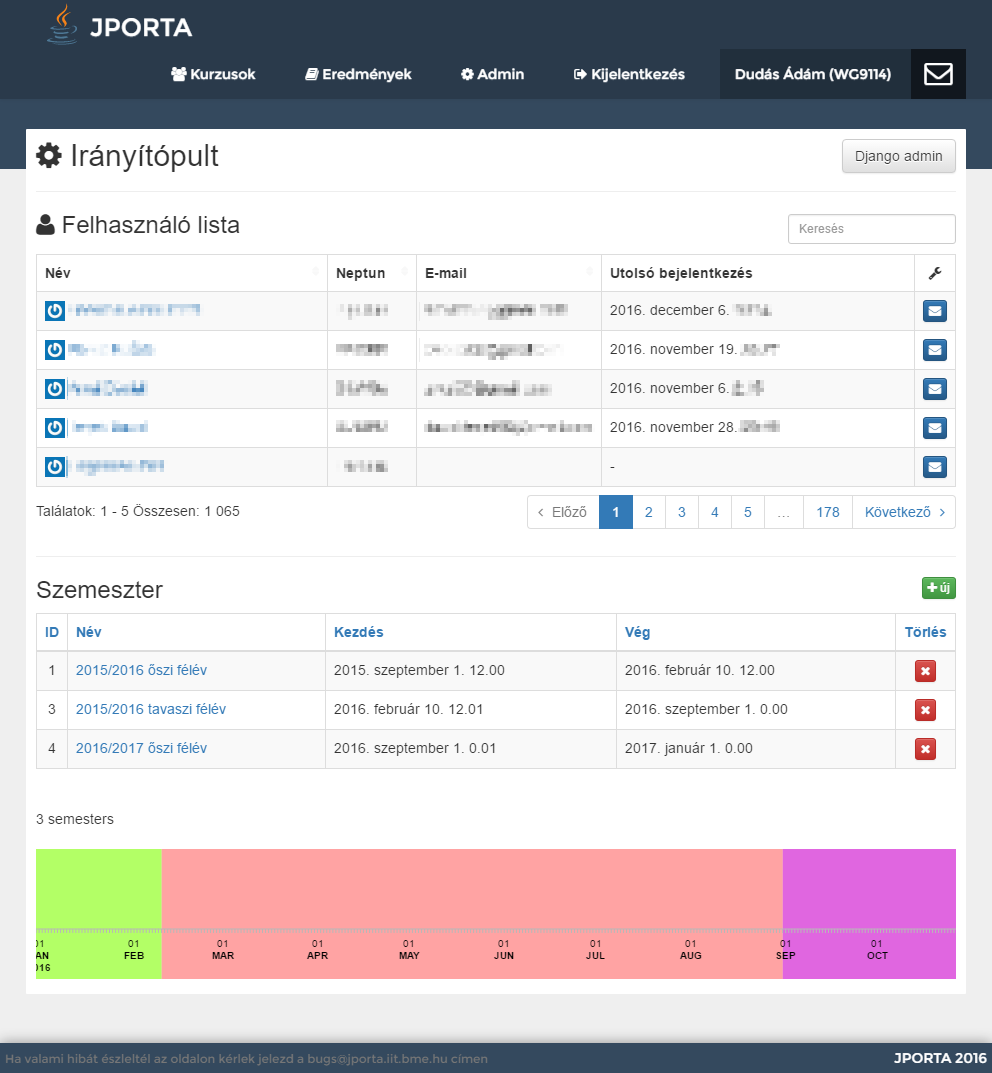
\includegraphics[width=\textwidth]{figures/Jporta-management-dashboard}
    \caption{Irányítópult}
    \label{figure:jporta-management-dashboard}
\end{figure}

Végül térjünk vissza a közös, minden felhasználó számára rendelkezésre álló funkciók tárgyalásához.

% Üzenetküldés
Az összes felhasználó számára rendelkezésre áll továbbá egy beépített üzenetküldés funkció, amelynek segítségével anélkül tudnak egymásnak üzenni a felhasználók, hogy ismerniük kellene címzettük, címzettjeik e-mail címeit.
Minden felhasználó megtekintheti a beérkezett üzeneteit a portál dedikált felületén (\figref{jporta-inbox}), de ha rendelkezik megadott e-mail címmel, akkor az üzenetek erre a címre is továbbításra kerülnek, sőt, a rendszer érzékeli, ha a levelet egy külső levelezőben olvasta a felhasználó, és azt belül is olvasottnak nyilvánítja.
\begin{figure}[h]
    \centering
    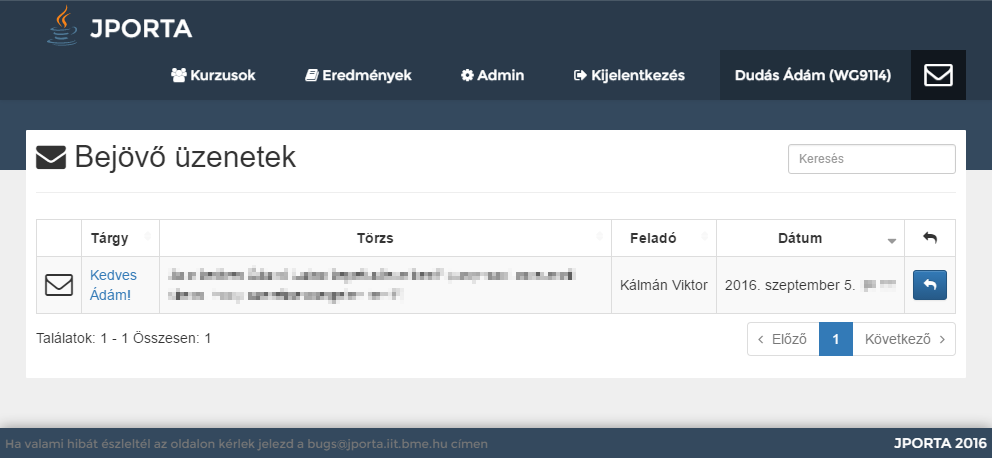
\includegraphics[width=0.95\textwidth]{figures/Jporta-inbox}
    \caption{Bejövő üzenetek}
    \label{figure:jporta-inbox}
\end{figure}
A tárgyért felelős oktatók a tárgy oldalán található \textit{Üzenetek} fül alatt akár az egész kurzusnak vagy bizonyos kurzuscsoportoknak is küldhetnek üzeneteket (\figref{jporta-course-messages}).
Ehhez hasonlóan a kurzuscsoportok oktatói is tudnak üzenetet küldeni saját csoportjaiknak.
\begin{figure}[h]
    \centering
    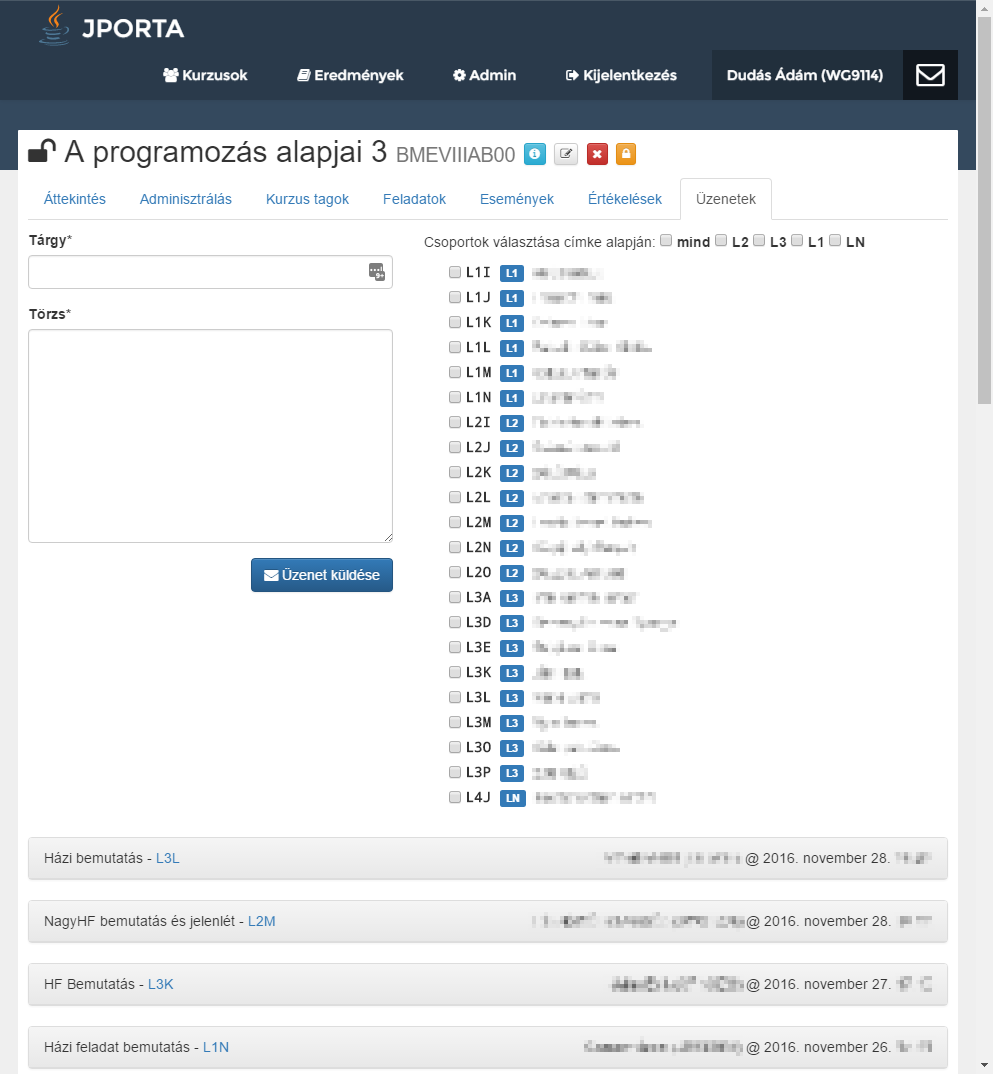
\includegraphics[width=0.95\textwidth]{figures/Jporta-course-messages}
    \caption{Kurzus szintű üzenetküldés}
    \label{figure:jporta-course-messages}
\end{figure}

% Profil
Végül, minden felhasználó rendelkezik egy profillal, ahol a fontosabb információk találhatóak meg (név, e-mail cím, profilkép, utolsó bejelentkezés ideje), és egy személyes beállítások oldallal, ahol kiválaszthatja az általa használni kívánt nyelvet és módosíthatja profilképét.